We test and validate our Autoencoder SINDy framework implementation by considering a Lorenz system and a non-linear pendulum as in \textcite{Champion_2019}. Like \textcite{Champion_2019}, our goal is to rediscover the original dynamics of the systems from high-dimensional data. 
To do so, we first generate the data using traditional methods, before attempting to rediscover the dynamics using our Autoencoder SINDy implementation.


\subsection{Data Generation}

This section describes the process used to generate datasets for training and evaluating the autoencoder SINDy framework, specifically focusing on the Lorenz system, and the nonlinear pendulum. Additionally, we discuss the transformation of the simulated data into a high-dimensional dataset which tests the framework's ability to discover the underlying low-dimensional dynamics.


\subsubsection{Lorenz System}
Introduced by Edward Lorenz in 1963 \cite{lorenz1963deterministic}, the Lorenz system is a simplified mathematical model for atmospheric convection, represented by a set of three ordinary differential equations (ODEs):
\begin{equation}
\begin{aligned}
    \dot{x} &= \sigma (y - x), \\
    \dot{y} &= x (\rho - z) - y, \\
    \dot{z} &= x y - \beta z,
\end{aligned}
\label{eq:lorenz}
\end{equation}
where the parameters $\sigma$, $\rho$, and $\beta$ are typically set to 10, 28, and $8/3$, respectively. These equations exhibit chaotic solutions for certain parameter values and initial conditions, making them a classic example of a system displaying sensitive dependence on initial conditions.


\begin{figure}[!htbp]
    \centering
    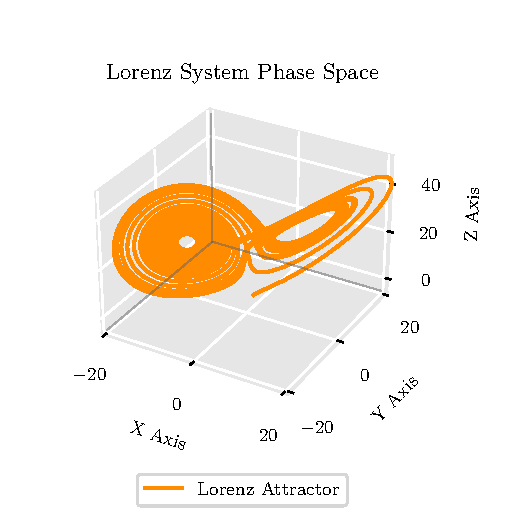
\includegraphics[width=0.48\textwidth]{project_2/images/lorenz_static.pdf}
    \caption{The Lorenz system's chaotic trajectory from initial conditions [1, 1, 1], depicting the typical butterfly-shaped attractor.}
    \label{fig:lorenz}
\end{figure}

% \begin{figure}
%     \centering
%         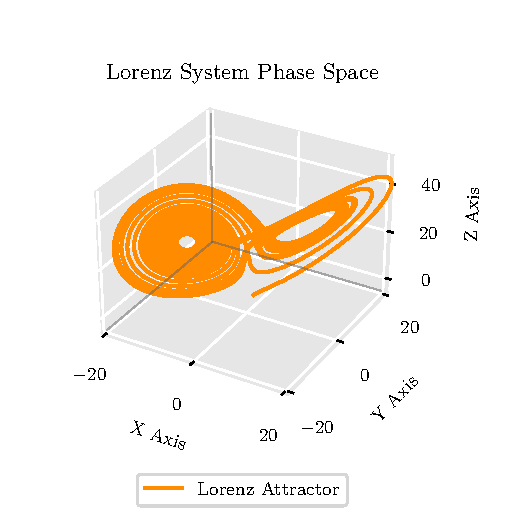
\includegraphics[width=0.48\textwidth]{project_2/images/lorenz_static.pdf}
%         \label{fig:lorenz}
%         % \caption{Lorenz System Trajectory Near a Stable Orbit: This plot illustrates the trajectory of the Lorenz system starting from initial conditions close to a stable orbit within the attractor. The purpose of these conditions is to verify the stability and precision of the numerical solutions under near-ideal circumstances.}
%     \caption{The Lorenz system's chaotic trajectory from initial conditions [1, 1, 1], depicting the typical butterfly-shaped attractor.}
%     \label{fig:init_dynamical_systems}
% \end{figure}
% \begin{figure}
%     \centering
%     \subfigure{
%         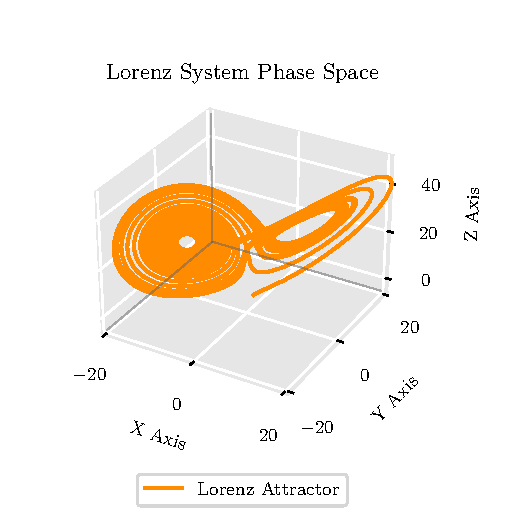
\includegraphics[width=0.48\textwidth]{project_2/images/lorenz_static.pdf}
%         \label{fig:lorenz}
%         % \caption{Lorenz System Trajectory Near a Stable Orbit: This plot illustrates the trajectory of the Lorenz system starting from initial conditions close to a stable orbit within the attractor. The purpose of these conditions is to verify the stability and precision of the numerical solutions under near-ideal circumstances.}
%     }
%     \caption{The Lorenz system's chaotic trajectory from initial conditions [1, 1, 1], depicting the typical butterfly-shaped attractor.}
%     \label{fig:init_dynamical_systems}
% \end{figure}

\subsubsection{Initial Conditions for the Lorenz Dataset}
We follow the method used by \textcite{Champion_2019} to generate initial conditions using a uniform distribution within set bounds for each variable.
\begin{equation}
\begin{aligned}
    x &\sim \mathcal{U}(-20, 20), \\
    y &\sim \mathcal{U}(-30, 30), \\
    z &\sim \mathcal{U}(5, 50).
\end{aligned}
\end{equation}
These ranges are chosen to sufficiently cover the phase space, ensuring a diverse set of trajectories for robust model training and evaluation. The datasets consist of 2048 initial conditions for training, 20 for validation, and 100 for out-of-distribution testing, providing a comprehensive basis for model assessment across a range of system states.




\subsubsection{Numerical Integration of the Lorenz Equations}
To solve the Lorenz system's differential equations, we employ the Runge-Kutta 45 (RK45) method, implemented via the \texttt{solve\_ivp} function from the \textit{SciPy} library and enhanced through JAX for execution on GPU platforms. This method is selected for its adaptive step-size control, balancing computational efficiency with the accuracy required to capture the system's chaotic dynamics accurately. Gaussian noise of strength \(1 \times 10^{-6}\) is added to the training data to simulate measurement inaccuracies and test the resilience of our modeling approach under simulated realistic conditions. The integration is performed over a linearly spaced time interval, \([0,5]\), with 100 steps yielding a high-resolution timestep, ensuring that the chaotic trajectories are finely detailed.\\

For the Lorenz system, initialized at \(x=y=z=1\), the RK45 method accurately captures the chaotic butterfly trajectories that characterize this system's sensitive dependence on initial conditions \cite{lorenz1963deterministic}.

\subsubsection{High-Dimensional Data Transformation of the Lorenz data}

The transformation of the ``low''-dimensional simulated Lorenz system's trajectory data into a high-dimensional space is achieved through the application of Legendre polynomials.
This transformation is central to testing the effectiveness of the autoencoder SINDy framework, and allows us to assess the framework's ability to reconstruct low-dimensional dynamics and reveal the fundamental laws that govern these systems; thus, verifying its robustness and adaptability \cite{Champion_2019}.\\

The transformations is as follows; the first three polynomials are used to linearly transform the system's variables, while the next three are used to introduce nonlinearities by transforming the cubic powers of the variables:
\begin{equation}
\begin{aligned}
    \mathbf{x}_i(t) &= \sum_{j=0}^{2} P_j(\mathbf{y}) \cdot \mathbf{z}_{ij}(t) + \sum_{j=3}^{5} P_j(\mathbf{y}) \cdot \mathbf{z}_{ij}(t)^3,
\end{aligned}
\end{equation}
where \( \mathbf{P}_j \) are the Legendre polynomials evaluated over the spatial domain \([-1, 1]\), and \( \mathbf{z}_{ij}(t) \) is the state vector at time \( t \) for each initial condition \( i \). This transformation not only enriches the dataset but also challenges the framework to decode and learn the underlying dynamics effectively from complex, high-dimensional inputs.

\subsubsection{Lorenz Data Handling and Model Training, Evaluation and Validation}
The high-dimensional data generated through this transformation are batched and processed using a combination of JAX utilities and custom data loaders designed to optimize computational efficiency on GPU architectures. The model is trained over 10,001 epochs with an additional 1,001 epochs for fine-tuning to ensure thorough learning under various system conditions and noise levels. This extensive training regimen is critical for developing a robust model capable of predicting dynamics across both in-distribution and out-of-distribution scenarios, enhancing the model's practical applicability and reliability in real-world settings.\\

Throughout the training process, validation is conducted using a separate dataset with 20 initial conditions, ensuring that the model's performance is not only evaluated on its ability to fit the training data but also on its generalization to new, unseen scenarios. Further, out-of-distribution tests with 100 initial conditions provide a stringent assessment of the model's resilience and adaptability, crucial for its deployment in conditions where robustness is paramount.


\subsubsection{Pendulum System}
The simple pendulum, a fundamental system in classical mechanics, is described by the second-order differential equation where the angle \( z \) measures the deviation from the vertical. The dynamic equation is given by:
\begin{equation}\label{eq:pendel}
    \ddot{z} = -\sin(z),
\end{equation}
which represents a simplified model of a pendulum under the influence of gravity without damping or external forces. This model captures the essential characteristics of pendular motion and provides a basis for studying more complex behaviors in nonlinear dynamics.

\subsubsection{Initial Conditions for the Pendulum System}
We generate initial conditions uniformly distributed within specific bounds for the angular position \( z \) and angular velocity \( \dot{z} \):
\begin{equation}
\begin{aligned}
    z &\sim \mathcal{U}(-\pi, \pi), \\
    \dot{z} &\sim \mathcal{U}(-2.1, 2.1).
\end{aligned}
\end{equation}
These ranges ensure that the pendulum does not possess enough energy to complete a full revolution. 

We attempted to recreate the conditions of Champion et al.'s paper by initially simulating \autoref{eq:pendel} from 100 randomly chosen initial conditions. However, due to the constraints imposed by using JAX arrays and the resulting GPU memory issues from handling such a large dataset, we adjusted our methodology. Consequently, we scaled down the number of simulations to 50 initial conditions for training and 10 for validation. Each simulation covers a time interval from 0 to 10 seconds at increments of 0.02 seconds, allowing us to effectively capture the dynamics of the system while managing computational resources efficiently.

\subsubsection{High-Dimensional Data Transformation of the Pendulum System}
To facilitate the study of the pendulum in the autoencoder-SINDy framework, we transform its one-dimensional angular data into a two-dimensional representation that mimics a visual observation of the pendulum's motion. This transformation is implemented as per the method described in the appendix of Champion's paper \cite{Champion_2019}, creating synthetic video of the pendulum in two spatial dimensions by generating high-dimensional snapshots given by:

\begin{equation}
\begin{split}
    x(y_1, y_2, t) &= \exp\left(-20\left((y_1 - \cos(z(t) - \frac{\pi}{2}))^2 \right. \right. \\
    &\quad \left. \left. + (y_2 - \sin(z(t) - \frac{\pi}{2}))^2\right)\right),
\end{split}
\end{equation}

where \(y_1\) and \(y_2\) span a discretized grid in the range \([-1.5, 1.5]\) with 51 grid points in each dimension, resulting in snapshots \(x(t) \in \mathbb{R}^{2601}\). This transformation not only enriches the input features but also provides a novel way to apply autoencoder frameworks for learning the underlying dynamics from visually interpretable data. The high-dimensional snapshots capture the pendulum's position over time, creating a detailed visual dataset that facilitates the application of image-based learning techniques.

\subsection{Optimization}
As stated, we employ the sequential thresholding least squares \cite{Brunton_2016} approach to training our SINDy Autoencoder.  

To optimize the least squares approach, we utilize the \textsc{ADAM} optimizer, originally proposed by \textcite{Adam}. \textsc{ADAM}, derived from adaptive moment estimation, is a gradient descent algorithm relying on first and second moments of the gradient to determine its descent direction. The full algorithm is displayed in \autoref{algo:ADAM}.
\begin{figure}[h]
    \begin{algorithm}[H]
    \caption{\textsc{ADAM}. $g^2$ denotes the elementwise square. $\beta_1,\beta_2\in [0,1) $ are hyperparameters controlling the decay rates of the moments. $\alpha$ is the learning rate, and $\epsilon>0$ is a numerical stabilizer. 
    The gradient is taken with respect to the autoencoder and SINDy parameters.}
    \label{algo:ADAM} 
       \begin{algorithmic}
        \State \( g_{k} \gets \nabla\mathcal{L} \)
        \State \(m_k \gets \beta_1 m_{k-1} + (1-\beta_1)g_k\) \Comment{\nth{1} order moment estimate}
        \State \(v_k \gets \beta_2 m_{k-1} + (1-\beta_2)g_k^2\)\Comment{\nth{2} order moment estimate}
        \State \(\hat{m_k} \gets \frac{m_k}{1-\beta_1^k}\)\Comment{bias correction}
        \State \(\hat{v_k} \gets \frac{v_k}{1-\beta_2^k}\)\Comment{bias correction}
        \State \(\theta_k \gets \theta_{k-1} - \alpha \frac{ \hat{m_k}}{\sqrt{\hat{v_k}+ \epsilon}}\)\Comment{Paramter update}
        \end{algorithmic}
    \end{algorithm}
\end{figure}


\textsc{ADAM} has become the de-facto optimization algorithm for many modern machine learning tasks, and it is applied extensively in the original Autoencoder SINDy paper \cite{Champion_2019}. Nevertheless, it is perhaps not suited to the non-differentiable $L_1$ terms in SINDy formulation, nor to sequential thresholding which periodically changes the loss landscape. We will explore these limitations further in the discussion 

\subsection{Technical Details}
We used \verb|JAX| \cite{jax2018github}, which is a library for automatic differentiation that allows for high-speed computations on both CPU and GPU which significantly speeds up large-scale model training. \verb|JAX| enables automatic differentiation through a variety of techniques, facilitating gradient-based optimization methods. Its ability to seamlessly handle large tensor operations and its compatibility with NumPy API which streamlines our development process. 

We also used \verb|Flax| \cite{Flax2020github} which is built on top of \verb|JAX| for implementing the SINDy Autoencoder framework. \verb|Flax| simplifies model definition, training, and evaluation by offering a layer of abstractions for model architectures. \verb|Flax|’s modular design allows rapid experimentation with various model configurations. The \textsc{ADAM} optimizer is implemented through the \verb|Optax| \cite{deepmind2020jax} optimization library for \verb|JAX|. 

Note that the baseline framework is based on that of \textcite{lippe2024}, although several modifications were made to improve SINDy Autoencoder specific performance. 

\subsubsection{Hardware}
We ran our simulations on the ML nodes at the University of Oslo\cite{uio_ml_nodes}, and on the GPUs available through Google Colab \cite{googlecolab}. 
The simulations were ran on the ML nodes at the University of Oslo, and 
